% siminos/spatiotemp/chapter/resistors.tex
% $Author: predrag $ $Date: 2021-12-24 01:25:20 -0500 (Fri, 24 Dec 2021) $

\section{Resistor networks}
\label{sect:resistors}

\begin{description}

\item[2017-09-11 Predrag]
A textbook:
Blanchard and Volchenkov\rf{BlaVol11}
{\em Random Walks and Diffusions on Graphs and Databases},
\CBlibrary{BlaVol11}; Chapter~6 {\em Random walks and electric resistance
networks}. They cite Doyle and Snell 1984; Tetali 1991; Chandra et al.
1996; Bollobas 1998 (have not looked at any of these).

They define the discrete representation of the Laplace
operator on a lattice in their eq.~(4.22). The matrix (4.38) corresponds
to the normalized Laplace operator.

``
It was established in Tetali (1991) and Chandra et al. (1996) that the
effective resistance might be interpreted as the expected number
of times a random walker visits all nodes of the network in a random
round trip from i to j and back.
''

\item[2020-01-10 Predrag]
A textbook:
A very pedagogical, down to earth textbook:
Pozrikidis\rf{Pozrikidis14}
{\em An introduction to grids, graphs, and networks},
\CBlibrary{Pozrikidis14} discusses this in
Chap.~6 {\em Network performance}. In part based on
Wu\rf{Wu04}, cited below. My notes are bellow, search for
{\bf 2020-01-10 Predrag}.

\item[2020-01-13 Predrag]
A textbook:
Grimmett\rf{Grimmett09} {\em Probability on Graphs: Random Processes on
Graphs and Lattices}, \CBlibrary{Grimmett09}.
Not sure we need this now, but it is a modern stat mech book on
percolation, Schramm–L\"owner evolution, Gibbs states and Markov fields,
the Ising and Potts models.

Chapter 1 is devoted to the relationship between random walks (on graphs)
and electrical networks. This leads to the Thomson and Rayleigh
principles, and thence to a proof of P\'olya's theorem.

\bigskip
Early papers are

Venezian\rf{Venezian94}
{\em On the resistance between two points on a grid}

 Atkinson and van Steenwijk\rf{AtkSte99}
{\em Infinite resistive lattices}

leading to much cited:

Cserti\rf{Cserti00} {\em Application of the lattice {Green's} function for
calculating the resistance of an infinite network of resistors}:

In the network of resistors it is assumed here that the resistances
of all the edges of the hypercube are the same, say
$R$. The goal is to find the resistance
between the origin and a given lattice point of the infinite
hypercube. Ohm's and Kirchhoff's laws for potential at a lattice site
are expressed in terms of the lattice Laplacian.
To find the resistance one solves a
Poisson-type equation by using the lattice
Green's function.

The 1\dmn\ case, his eq.~(23) is very simple.

The energy-dependent lattice Green's function of the tight-binding
Hamiltonian for a square lattice, his eq.~(30), has energy $E$ playing
the role of our stretching parameter $s$.

He does the actual derivations on finite $d$-tori, but only as a step
preliminary to taking the infinite-lattice limit; no actual calculations
for finite $d$-tori.

[...] The value of G(0,0,0) was evaluated for the first time by
Watson~[21] and subsequently by Joyce~[22] in a closed form in terms of
the complete elliptic integral of the first kind
% [3] P. G. Doyle and J. L. Snell, Random Walks and Electric Networks,
%       The Carus Mathematical Monograph, Series 22
%       The Mathematical Association of America, USA, 1984, pp. 83–149.
% [21] G. N. Watson, ``Three triple integrals,''
%       Q. J. Math. 10, 266–276 ~1939
%[22] G. S. Joyce, ``Lattice Green function for the simple cubic lattice,''
%       J. Phys. A 5, L65–L68 ~1972!.
%[23] M. L. Glasser and I. J. Zucker,
%       ``Extended Watson Integrals for Cubic Lattices,''
%       Proc. Natl. Acad. Sci. USA 74, 1800–1801 ~1977!.
\beq
K(k) = \int_0^{\pi/2} d\theta \frac{1}{\sqrt{1-k^2\sin^2\theta}}
\ee{Cserti00(38)}
It is worth
mentioning that a simpler result was obtained by Glasser and
Zucker~[23] (see also Doyle and Snell's book\rf{DoySne00}),
\arXiv{math/0001057}, who calculated
the integrals in terms of gamma functions:
\beq
2\,G(0,0,0) = \frac{\sqrt{3}-1}{96\pi^3}\Gamma^2(1/24)\Gamma^2(11/24)
\,.
\ee{Cserti00(39)}
Predrag finds this form intriguing, as he expects symmetry factorizations
in the spirit of \refeq{AABHM99-46a}.

Glasser and Montaldi~[27] gave other useful integral representations
of the lattice Green's function for the hypercubic lattice
for arbitrary dimension $d$.
% [27] M. L. Glasser and E. Montaldi,
%        ``Staircase polygons and recurrent lattice walks,''
%        Phys. Rev. E 48, R2339–R2342 ~1993!.
It was shown by Joyce~[22] that the function G(E;0,0,0) can
be expressed in the form of a product of two complete elliptic
integrals of the first kind. (Predrag: presumably a symmetry factorization.)



This work is continued in \refref{CsSzDa11}:

\item[2019-11-04 Predrag]
Cserti, Sz{\'{e}}chenyi and D{\'{a}}vid\rf{CsSzDa11}
{\em Uniform tiling with electrical resistors}:
``
The resistance between two arbitrary nodes of a network of resistors is
studied when the network is perturbed by connecting an extra resistor
between two arbitrary nodes in the perfect lattice. The lattice Green's
function and the resistance of the perturbed network are expressed in
terms of those of the perfect lattice by solving Dyson's equation. A
comparison is carried out between numerical and experimental results for
a square lattice.
''

The electric resistance between two arbitrary nodes on any infinite
lattice structure of resistors that is a periodic tiling of space is
obtained, using the lattice Green's function
of the Laplacian matrix associated with the network.
The method can be extended to the random walk problem or to
electron dynamics in solid state physics.
The results may be used to calculate the wavefunctions at the lattice
points for complicated lattice structures.

I do not think we need this paper at the present stage - understanding
`undecorated' square lattice is all we need...

%\item[2019-11-04 Predrag]
%Giaro [5] calculated the resistance between two arbitrary points in the
%infinite square lattice networks that utilizes the basic properties of
%Fourier series.



\item[2019-11-01 Predrag]
Introduction of Owaidat, Asad and Tan\rf{OwAsTa19} {\em Resistance
computation of generalized decorated square and simple cubic network
lattices} has a very exhaustive lattice Green functions literature
discussion, starting with

Kirchhoff\rf{Kirchhoff1847} {\em {\"U}eber die Aufl{\"o}sung der
Gleichungen, auf welche man bei der Untersuchung der linearen Vertheilung
galvanischer Str{\"o}me gef{\"u}hrt wird}, which, weirdly enough, reminds
me that I've computed for my PhD\rf{CviKin74a} the determinants for QED
that we here seek to compute for a much simpler lattice problem.

Their work follows the Green's function theory presented by
Cserti\rf{Cserti00}. They say that the lattice Green functions are
usually evaluated as the elliptic integrals \refeq{Cserti00(38)} or by
recurrence relations methods.

They do display a determinant of a Laplacian, eq.~(B.11) in their Appendix
B.~{\em The matrix elements of the Green's function for the generalized
decorated simple cubic lattice}, but it is a determinant of a
single Fourier mode (in each of the three directions of a cubic lattice). Han
has the analogue for the square lattice - what we do not have is the
product formula, in which all eigenvalues (cosines, etc) average out, and
all that is left is a polynomial in $s$

\item[2019-11-04 Predrag]
Jafarizadeh, Sufiani and Jafarizadeh\rf{JaSuJa07} {\em Calculating
two-point resistances in distance-regular resistor networks}
provide an algorithm for the calculation of the resistance between two
arbitrary nodes in an arbitrary distance-regular resistor network.

Past efforts have been focused mainly on infinite lattices, with little
attention paid to finite networks. They present a general formulation for
computing two-point resistances in finite networks.

Their starting point is the Laplacian matrix associated with a network.
The Laplacian is a matrix whose off-diagonal entries are the conductances
connecting pairs of nodes. Just as in graph theory where everything about
a graph is described by its adjacency matrix (whose element is 1 if two
vertices are connected and 0 otherwise), everything about an electric
network is described by its Laplacian.

The two-point resistances on a network depend only on the Stieltjes
function $G_\mu(x)$ corresponding to the network. The Stieltjes function
corresponding to an infinite network possesses a unique representation as
an infinite continued fraction. In the cases for which the parameters
iterate themselves after some finite steps, one can find a closed form
for the infinite continued fraction. This situation takes place, for
instance, in the infinite line network. But in most cases, this situation
dose not occur and one cannot obtain a closed form for the Stieltjes
function of the network.

\item[2019-11-04 Predrag]
Wu\rf{Wu04} {\em Theory of resistor networks: the two-point resistance}
is a foundational paper, where a theory to calculate the
resistance between arbitrary nodes for a finite lattice of resistors is
given in terms of the eigenvalues and eigenvectors of the graph Laplacian
matrix.

Wu gives a closed-form expression,  his eq.~(43), for the resistance
$R^{[L\!\times\!T]}_{z_1 z_2}$ of a finite square lattice between
nodes $z_1=(x_1,y_1)$ and $z_2=(x_2,y_2)$ for free, periodic and
cylindrical boundary conditions.

%%%%%%%%%%%%%%%%%%%%%%%%%%%%%%%%%%%%%%%%%%%%
\begin{figure}
  \centering
  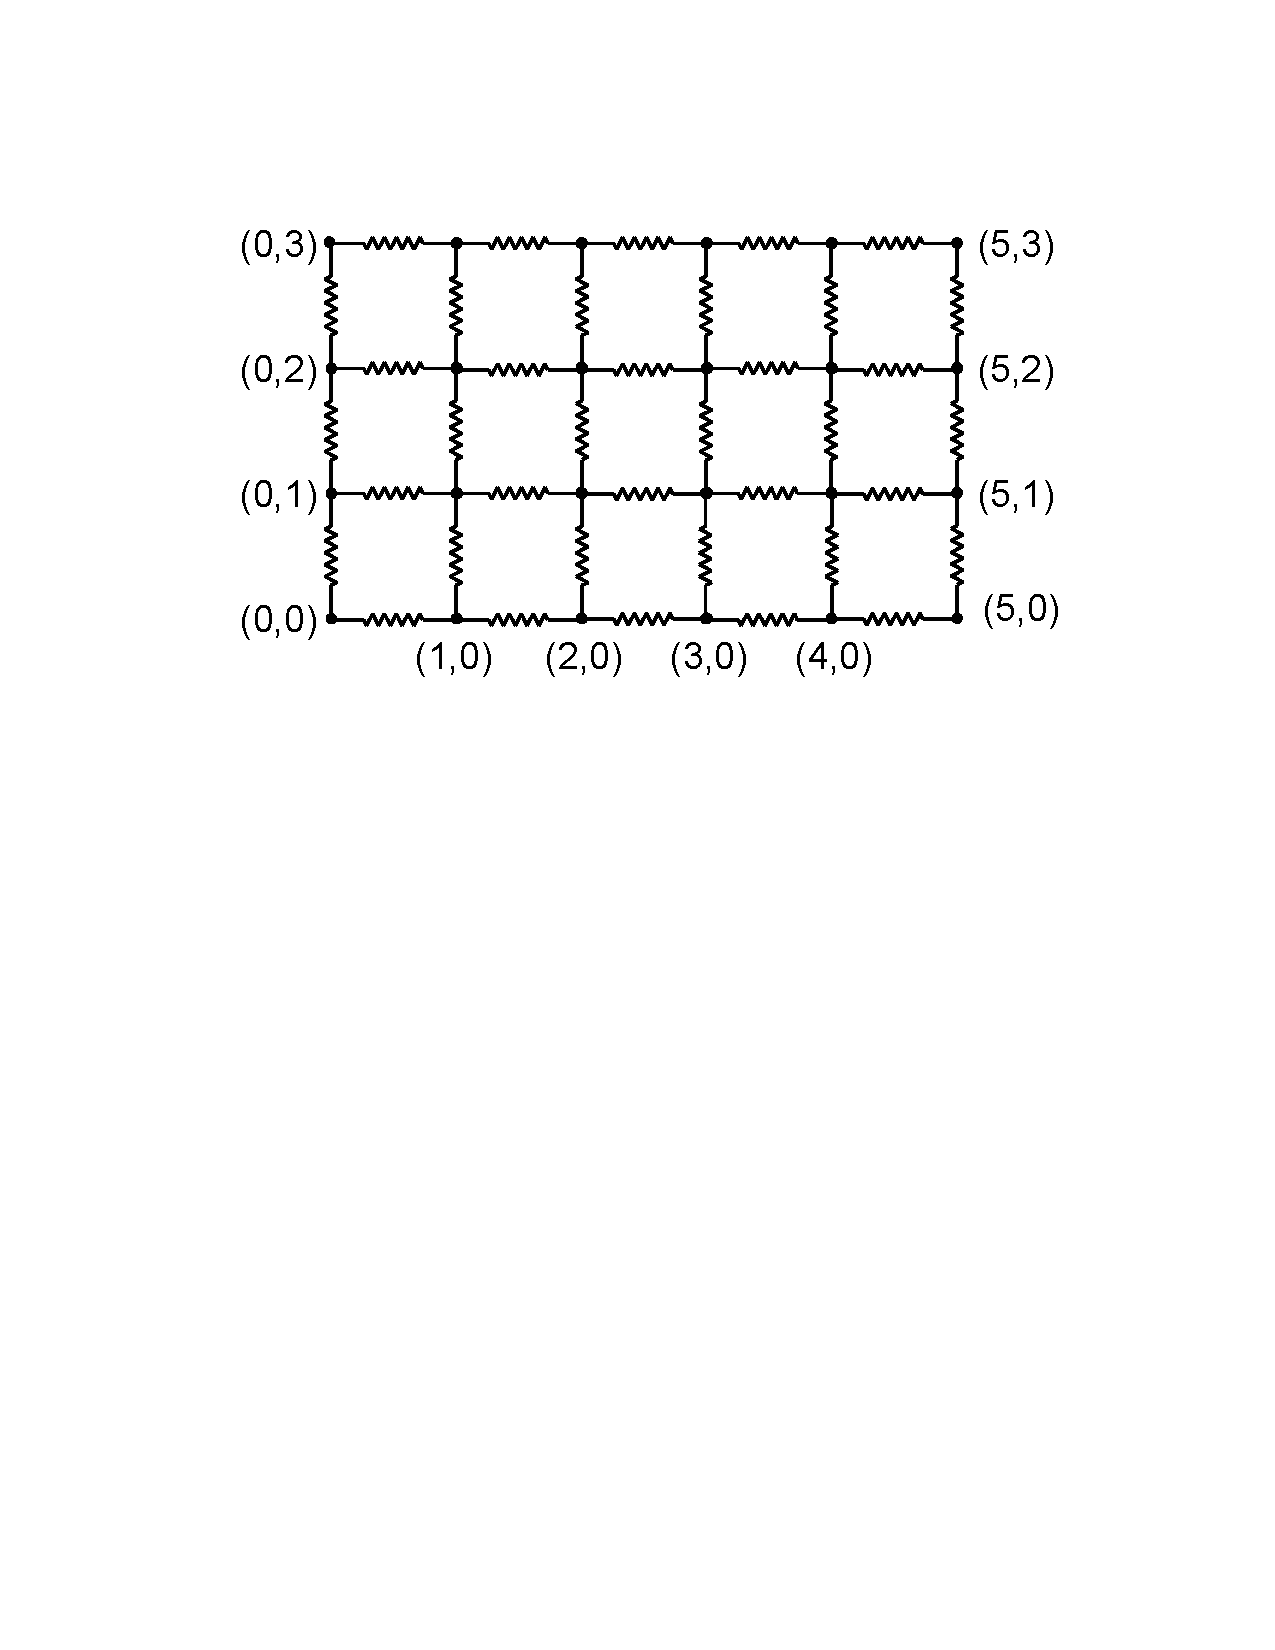
\includegraphics[width=0.60\textwidth]{Wu04fig4}
  \caption{\label{Wu04fig4}
A $[5\!\times\!4]$ rectangular resistor network:
resistors with resistances $r$ and $s$ on edges of the network in,
respectively, horizontal and vertical directions.
  }
\end{figure}
%%%%%%%%%%%%%%%%%%%%%%%%%%%%%%%%%%%%%%%%%%%%

The paper is very clear and explicit, with many examples, including the
1\dmn\ periodic chain (sect.~{\em 3.2. Periodic boundary conditions}) and
the doubly periodic $[L\!\times\!T]$ square lattice, his sect.~{\em 5.
Two-dimensional network} and \reffig{Wu04fig4}. His eq.~(43) gives the
resistance between  nodes $z_1=(x_1, y_1)$
and  $z_2=(x_2, y_2)$
 \bea
R^{[L\!\times\!T]}_{z_1 z_2}
%R_{\{M\times N\}}^{\rm per} ({\bf r}_1,{\bf r}_2)
&=&  {\sum_{m=0}^{M-1}\sum_{n=0}^{N-1}} _{(m,n) \not= (0,0)}
\frac{\Big|\psi_{(m,n);(x_1,y_1)} - \psi_{(m,n);(x_2, y_2)}\Big|^2 }{\lambda_{(m,n)}} \nonumber \\
%&=& \frac{1}{N} R_{\{M\times 1\}}^{\rm per}(x_1,x_2)
%+  \frac{1}{M} R^{\rm per}_{\{N\times 1\}}(y_1,y_2)\nonumber \\
&=& \frac{r}{N} \Bigg[\,\Big| x_1 -x_2 \Big| -\frac{(x_1-x_2)^2}{M}
\Bigg] + \frac{s}{M}\Bigg[\,\Big| y_1 -y_2 \Big| -\frac{(y_1-y_2)^2}{N}
\Bigg] \nonumber \\
&+& \frac{1}{MN} \sum_{m=1}^M \sum_{n=1}^N
\frac{1- \cos \Big[2(x_1-x_2)\theta_m+2(y_1-y_2)\phi_n \Big]}
 {r^{-1}\big(1-\cos 2\theta_m \big)+s^{-1}\big(1-\cos 2\phi_n \big)} ,\nonumber \\
&& \hskip 2cm
\label{Wu04:RR}
\eea
% where  the two terms in the second line are given by (\ref{R1Dper}).
The result depends only on the differences
$\big|x_1-x_2\big|$ and $\big|y_1-y_2\big|$, as it should
by translational invariance.
This is a double sum over Fourier modes, and I see no determinant
calculation where these are summed over and what remains is some sensible
polynomial.

However, his sect.~{\em 10.
Summation and product identities} might be just what we need:

He shows that
\bea
 F_N(\ell) &=& \frac{1}{N} \sum_{n=1}^{N-1} \frac{1-\cos (\ell \phi_n)}{1-\cos \phi_n}
\continue
            &=& |\ell| - \frac{1}{N} \Bigg(\frac{\ell^2 +|\ell|}{2}
                       - \Bigg[\frac{|\ell|}{2}\Bigg] \Bigg)
\label{Wu04:F1}
\eea
where $[x]$ denotes the integral part of $x$.
Similarly
\[
G_N(\ell)=
 \frac{1}{N} \sum_{n=1}^{N-1} \frac{1-\cos (2\ell \phi_n)}{1-\cos 2\phi_n}
\,.
\]
\medskip
is evaluated as a special case of the identity
(\ref{Wu04:I2}), using
the recursion relation
\[
G_N(\ell)-G_N(\ell-1) = 1- \frac{1}{N} \big({2\ell -1}\big) \nonumber
\]
which yields
\beq
G_N(\ell) = \big|\ell\big| - \ell^2/N
\,.
\ee{Wu04:GN}




\medskip
\noindent
{\it Proposition: Define
\[
I_\alpha (\ell) =  \frac{1}{N} \sum_{n=0}^{N-1} \frac{\cos\big(\alpha\,\ell\, \frac{n\pi}{N} \big)}
  {\cosh \lambda -\cos \big(\alpha \,\frac{n\pi}{N} \big)}, \hskip1cm \alpha=1,2
\,.
\]
Then the following identities hold for $\lambda \geq 0$, $N=1,2,\cdots,$ }
 \bea
 I_1(\ell)  &=&\frac{\cosh(N-\ell)\lambda}{(\sinh \lambda) \sinh (N\lambda)}  + \frac{1}{N} \Bigg[ \frac{1}{\sinh^2\lambda}
  + \frac{1-(-1)^\ell}{4\cosh^2(\lambda/2)}\Bigg],\ 0 \leq \ell< 2N,\nonumber \\
  \label{Wu04:I1} \\
 I_2(\ell) &=&\frac{\cosh \big(\frac{N}{2} - \ell\big) \lambda}{(\sinh \lambda) \sinh (N\lambda/2)}\, ,
          \hskip 3.2cm 0 \leq \ell< N
\,.
 \label{Wu04:I2}
 \eea
\noindent
Remarks:

\medskip
3. In the  $N\to\infty$ limit both  (\ref{Wu04:I1}) and  (\ref{Wu04:I2}) become the  integral
\[
\frac{1}{\pi} \int_0^\pi \frac{\cos (\ell \theta)}{\cosh \lambda - \cos \theta}  d\,\theta
= \frac{e^{-\ell \lambda}}{\sinh \lambda}  \quad \quad \ell \geq 0 .
\]

\medskip
4.  Set $\ell = 0$ in (\ref{Wu04:I1}), multiply by $\sinh \lambda$ and integrate over $\lambda$, we obtain the product
identity
\beq
\prod_{n=0}^{N-1} \bigg( \cosh \lambda -\cos \frac{n\pi}{N}\bigg)
= (\sinh N \lambda) \tanh ( {\lambda}/ 2).
\ee{Wu04:prod}

\medskip
5. Set $\ell = 0$ in (\ref{Wu04:I2}), multiply by $\sinh \lambda$ and integrate over $\lambda$.  We obtain the product
identity
\beq
\prod_{n=0}^{N-1} \bigg( \cosh \lambda -\cos \frac{2n\pi}{N}\bigg) = \sinh^2 ( {N\lambda}/ 2).
\ee{Wu04:prod1}


\medskip
\noindent
 Proof:

\medskip
Introduce
\bea
S_\alpha(\ell) =
\frac{1}{N} \sum_{n=0}^{N-1} \frac{\cos(\ell\, \theta_n)}
  {1+a^2 -2a\cos \theta_n}, \hskip 1cm a<1 , \quad \alpha=1,2 \label{Wu04:SL}
\eea
so that
\beq
I_\alpha(\ell) = 2\, a\, S_\alpha(\ell), \hskip1cm  a=e^{-\lambda}.
\eeq
 It is readily seen that we have the identity
\beq
S_\alpha(1) = \frac{1}{2a} \Big[ (1+a^2) S_\alpha (0)-1\Big]. \label{Wu04:S10}
\eeq

\medskip
\noindent
1. Proof  of (\ref{Wu04:I1}):

\medskip
First we evaluate $S_1(0)$ by carrying
 out the following summation, where ${\cal R}$e denotes the real part,
in two different ways.  First we have
\bea
{\cal {R}}e\,
\frac{1}{N} \sum_{n=0}^{N-1}
  \frac{1}{ 1- a\, e^{i\theta_n}}
 &=& {\cal {R}}e\, \frac{1}{N} \sum_{n=0}^{N-1}
  \frac{1-a \, e^{-i\theta_n}}{\Big| 1- a\, e^{i\theta_n}\Big|^2} \nonumber \\
&=& \frac{1}{N} \sum_{n=0}^{N-1} \frac{1-a \cos \theta_n}{1+a^2-2a\cos \theta_n} \nonumber \\
&=& S_1(0) -a S_1(1) \nonumber \\
&=& \frac{1}{2} \Big[1+ (1-a^2)  S_1(0)\Big].  \label{Wu04:I11}
\eea
Secondly by expanding the summand we have
\bea
{\cal {R}}e\,\frac{1}{N} \sum_{n=0}^{N-1}
  \frac{1}{ 1- a\, e^{i\theta_n}}
={\cal {R}}e\,\frac{1}{N} \sum_{n=0}^{N-1} \sum_{\ell=0}^\infty a^\ell e^{i\ell n\pi/N}
 \nonumber
\eea
and carry out the summation over $n$
for fixed $\ell$.
  It is clear that all $\ell=$ even terms vanish except those with $\ell = 2 m N, m=0,1,2,...$
which yield $\sum_{m=0}^\infty a^{2mN} =1/(1-a^{2N})$.
For $\ell = $ odd $=2m+1,$ $m=0,1,2,...$ we have
\bea
{\cal {R}}e\, \sum_{n=0}^{N-1} e^{i(2m+1) n\pi/N}
   = {\cal {R}}e\,\frac{1-(-1)^{2m+1}}{1-e^{i(2m+1)\pi/N}} = 1 \nonumber
\eea
after making use of % (\ref{Wu04:12}),
\beq
{\cal R}e\,\Bigg( \frac{1}{1-e^{i\theta}} \Bigg)= \frac{1}{2}, \hskip1cm
 0<\theta <2\pi
 \,.
\ee{Wu04:12}
So the summation over $\ell=$ odd terms  yields
$N^{-1}\sum_{m=0}^\infty a^{2m+1} =a/N(1-a^{2})$, and  we have
\beq
{\cal {R}}e\, \sum_{n=0}^{N-1}\frac{1}{ 1- a\, e^{i\theta_n}}
   =  \frac{1}{1-a^{2N}} +\frac{a}{N(1-a^2)} \label{Wu04:I12}
\eeq
Equating (\ref{Wu04:I11}) with  (\ref{Wu04:I12})  we obtain
\beq
S_1(0) = \frac{1}{1-a^2} \Bigg[ \Bigg(\frac{1+a^{2N}}{1-a^{2N}}\Bigg)
  + \frac{2a}{N(1-a^2)} \Bigg]
  \,.
\label{Wu04:SN1}
\eeq

\medskip
To evaluate $S_1(\ell)$ for general $\ell$,  we
consider the summation
 \bea
{\cal {R}}e\,
\frac{1}{N}\sum_{n=0}^{N-1}
  \frac{1-\big(a\, e^{i \theta_n}\big)^\ell} { 1- a\, e^{i \theta_n}}
 &=& {\cal {R}}e\,
\frac{1}{N}\sum_{n=0}^{N-1}
  \frac{(1-a^\ell\, e^{i \ell \theta_n})(1-a\, e^{-i\theta_n})}
       {\big|1- a\, e^{i \theta_n}\big|^2}
\label{Wu04:I41}\\
&=&  S_1(0) - a S_1(1) - a^\ell S_1(\ell) +a^{\ell+1} S_1(\ell-1)
\,,
\nonumber
\eea
where the second line is obtained by writing out  the real part of the summand as in (\ref{Wu04:I11}).
 On the other hand, by expanding the summand we have
\bea
{\cal {R}}e\,
\frac{1}{N} \sum_{n=0}^{N-1}
  \frac{1-\big(a\, e^{i \theta_n}\big)^\ell} { 1- a\, e^{i \theta_n}} &=&
{\cal {R}}e\,
\frac{1}{N} \sum_{n=0}^{N-1} \sum_{m=0}^{\ell -1} a^m e^{i\pi m  n/N} \nonumber \\
&=& 1+{\cal {R}}e\,
\frac{1}{N} \sum_{m=1}^{\ell-1} a^m \Bigg(\frac{1-(-1)^m}{1-e^{i\pi m/N}} \Bigg) \nonumber \\
&=& 1+\frac{a(1-a^\ell)} {N(1-a^2)}, \quad \ell = {\rm even}< 2N \nonumber \\
&=& 1+\frac{a(1-a^{\ell-1})} {N(1-a^2)}, \quad \ell = {\rm odd} <2N
\,,
\label{Wu04:I42}
\eea
where again we have used (\ref{Wu04:12}).

\medskip
 Equating (\ref{Wu04:I42}) with (\ref{Wu04:I41}) and using
(\ref{Wu04:S10})   and (\ref{Wu04:SN1}),
 we obtain the recursion relation
\beq
S_N(\ell)-a\,S_N(\ell-1)=A\,a^{-\ell} +B_\ell
\ee{Wu04:Q}
 where
\bea
A =\frac{a^{2N}}{1- {a^{2N}} }, \hskip 1cm B_\ell = \frac{a^{(1+(-1)^\ell)/2} }{ N(1-a^2)} .
\eea

The recursion relation (\ref{Wu04:Q}) can be solved by standard means.  Define
 the generating function
\beq
G_\alpha(t) =\sum_{\ell =0}^\infty S_\alpha(\ell)\, t^\ell, \hskip1cm \alpha=1,2
\,.
\ee{Wu04:gen}
Multiply (\ref{Wu04:Q}) by $t^\ell$ and sum over $\ell$.  We obtain
\bea
(1-at)G_1(t) -S_1(0) = \frac{A\,a^{-1}t}{1-a^{-1}t} + \frac{t+at^2} {N(1-a^2)(1-t^2)}.
\eea
This leads to
\bea
G_1(t) &=& \frac{1}{1-at} \Bigg[ S_1(0) +\frac{A\,a^{-1}t}{1-a^{-1}t} +
\frac{t+at^2} {N(1-a^2)(1-t^2)} \Bigg] \nonumber \\
 &=&\frac{1}{(1-a^2)(1-a^{2N})} \Bigg[\frac{1}{1-at}
  +\frac{a^{2N} }{1-a^{-1}t} \Bigg] \nonumber \\
&&+\, \frac{1}{2N(1-a)^2(1-t)} -\frac{1}{2N(1+a)^2(1+t)},\nonumber
\eea
from which one obtains
\bea
S_1(\ell) &=& \frac{a^\ell +a^{2N-\ell}} {(1-a^2)(1-a^{2N})}
+ \frac{1}{2N(1-a)^2} - \frac{(-1)^\ell}{2N(1+a)^2} \nonumber \\
&=& \frac{a^\ell +a^{2N-\ell}} {(1-a^2)(1-a^{2N})}
+\frac{1}{2N} \Bigg[\frac{4a} {(1-a^2)^2} +\frac{1-(-1)^\ell}{(1+a^2)^2}\Bigg].
\eea
It follows that using
 $I_1(\ell) = 2\,a\, S_1(\ell)$
we obtain (\ref{Wu04:I1}) after setting $a=e^{-\lambda}$.

\medskip
\noindent
2. Proof of (\ref{Wu04:I2}):

\medskip
Again, we first evaluate $S_2(0)$ by carrying out the summation
\[
{\cal {R}}e\,
\frac{1}{N} \sum_{n=0}^{N-1}
  \frac{1}{ 1- a\, e^{i2\theta_n}}, \hskip1cm a<1
\]
in two different ways.  First as in
(\ref{Wu04:I11}) we have
\bea
{\cal {R}}e\,
\frac{1}{N} \sum_{n=0}^{N-1}
  \frac{1}{ 1- a\, e^{i2\theta_n}}
  = \frac{1}{2} \Big[1+ (1-a^2)  S_2(0)\Big], \label{Wu04:I21}
\eea
where $S_2(\ell)$ is defined in (\ref{Wu04:SL}).
 Secondly by expanding the summand we have
\beq
\frac{1}{N} \sum_{n=0}^{N-1}
  \frac{1}{ 1- a\, e^{i2\theta_n}}
=\frac{1}{N} \sum_{n=0}^{N-1} \sum_{\ell=0}^\infty a^\ell e^{i2\ell n\pi/N}
=\frac{1}{1-a^N}
\ee{Wu04:I22}
where by carrying out the summation over $n$
for fixed $\ell$ all terms in (\ref{Wu04:I12})
vanish except those with $\ell = m N, m=0,1,2,...$
 Equating
(\ref{Wu04:I22}) with (\ref{Wu04:I21})  we obtain
\bea
  S_2(0)= \frac{1}{1-a^2} \Bigg(\frac{1+a^N}{1-a^N} \Bigg) \label{Wu04:SN2}
\eea
and from (\ref{Wu04:S10})
\bea
S_2(1) = \frac{1}{1-a^N}. \nonumber
\eea
We consider next the summation
\beq
 {\cal {R}}e\,
\frac{1}{N} \sum_{n=0}^{N-1}
  \frac{1-\big(a\, e^{i2 \theta_n}\big)^\ell}{ 1- a\, e^{i2 \theta_n}} \hskip1cm a<1
  \,.
\ee{Wu04:I20}
Evaluating the real part of the summand directly as in (\ref{Wu04:I41}), we obtain
\bea
{\cal {R}}e\,
\frac{1}{N} \sum_{n=0}^{N-1}
  \frac{1-\big(a\, e^{i2 \theta_n}\big)^\ell}{1- a\, e^{i2 \theta_n}} =
  S_2(0) - a S_2(1) - a^\ell S_2(\ell) +a^{\ell+1} S_2(\ell-1).\label{Wu04:I23}
 \eea
   Secondly, expanding the summand in (\ref{Wu04:I20}) we obtain
\bea
\frac{1}{N} \sum_{n=0}^{N-1}
  \frac{1-\big(a\, e^{i2 \theta_n}\big)^\ell} { 1- a\, e^{i2 \theta_n}}
 &=& \frac{1}{N} \sum_{n=0}^{N-1}
  \sum_{m=0}^{\ell-1} a^m e^{i2\pi mn/N} \nonumber \\
&=& \frac{1}{N} \Bigg[ N + \sum_{m=1}^{\ell-1} \frac{1-e^{i2m\pi}}{1-e^{i2m\pi/N}}\Bigg] \nonumber \\
&=& 1 \hskip 2cm m<\ell \leq N . \label{Wu04:I24}
\eea
 Equating (\ref{Wu04:I24}) and (\ref{Wu04:I23}) and making use of (\ref{Wu04:SN2})
for $S_2(0)$, we obtain
\bea
S_2(\ell) -a S_2(\ell-1) = \frac{a^{N-\ell}}{1-a^N}  \label{Wu04:rec1}
\eea

The recursion relation (\ref{Wu04:rec1}) can be solved as in the above.
Define the generating function $G_2(t)$ by (\ref{Wu04:gen}).
 We find
\bea
G_2(t) &=&
\frac{1}{1-at}\Bigg[S_2(0) + \frac{a^{N-1}t}{(1-a^N) (1-a^{-1}t)} \Bigg] \nonumber \\
 &=& \frac{1}{(1-a^2)(1-a^{2N})} \Bigg[\frac{1}{ 1-at} + \frac{a^N}{ 1-a^{-1}t}\Bigg],
\eea
from which one reads off
\[
S_2(\ell) = \frac{a^\ell +a^{N-\ell}} {(1-a^2)(1-a^{2N})}.
\]
Using the relation $I_2(\ell) = 2\, a\, S_2(\ell)$ with $ a=e^{-\lambda}$, we obtain (\ref{Wu04:I2}).


\item[2019-11-04 Predrag]
Tzeng and Wu have extended this impedance networks, where the
Laplacian matrix has complex matrix elements; I think we do not care
about this at this time.


\item[2019-11-04 Predrag]
The corner-to-corner resistance and its asymptotic expansion for various
boundary conditions were calculated by Izmailian and Huang\rf{IzmHua10}
{\em Asymptotic expansion for the resistance between two maximally
separated nodes on an {$M$} by {$N$} resistor network}:
``
The computation of the asymptotic expansion of the corner to-corner
resistance, in other word the resistance between two maximally separated
nodes of a rectangular resistor network is of interest as its value
provides a lower bound to the resistance of compact percolation clusters
in the Domany-Kinzel model of a directed percolation [15]. ''

They take a $[\speriod{}\times\period{}]$ array, use a ton of funky
identities, and manage to reduce Wu's double sum \refeq{Wu04:RR} to a
single, highly non-obvious sum, their eq.~(33).
Then there are Kronecker's double series
expressed in terms of the complete elliptic integrals $K(s)$ and $E(s)$.

\item[2020-01-11 Predrag] Dienstfrey, Hang and Huang\rf{DiHaHu01} {\em
Lattice sums and the two-dimensional, periodic {Green's} function for the
{Helmholtz} equation}.
They compute the Green's function for the Helmholtz equation in two
dimensions with doubly periodic boundary conditions, on a fundamental
cell $[-1/2,12)^2$. I believe this is not relevant to us, it solves a
continuous problem over the unit cell, rather than a problem on discrete
lattice.

Due to the translation invariance, the Green's function has a convolution
structure,
\(
G(x,x_0)= G(y)
\,,\quad y=x-x_0
\in[-1,1)^2
\,.
\)
A periodic Helmholtz equation can be computed via the method of images
over the zeroth-order Hankel function of the first-kind. The sums can
also be evaluated by recognizing an identity between the so-called
`spectral' and `spatial' representations of $G$. For a square array,
there are symmetries which allow for further simplification.

\item[2020-01-10 Predrag]
Stewart and G{\"o}kaydin\rf{SteGok19}
{\em Symmetries of quotient networks for doubly periodic patterns on the
square lattice}, \CBlibrary{SteGok19}. Read for
\refsect{sect:fundDomHL}~{\em Reduction to the fundamental domain} that has still
to be completed.

\item[2020-01-10 Predrag]
A very pedagogical, down to earth textbook:
Pozrikidis\rf{Pozrikidis14}
{\em An introduction to grids, graphs, and networks},
\CBlibrary{Pozrikidis14}:

\emph{Graphs} are finite or infinite sets of vertices connected by edges in
structured or unstructured configurations.

Infinite \emph{lattices} and tiled surfaces are described by highly ordered graphs
parametrized by an appropriate number of indices.

\emph{Networks} consist of nodes connected by physical or abstract links
with an assigned conductance in spontaneous or engineered configurations.
In physical and engineering applications, networks are venues for
conducting or convecting a transported entity, such as heat, mass, or
digitized information according to a prevailing transport law.

\emph{Finite difference} and finite element \emph{grids} can be regarded
as networks whose link conductance is determined by the differential
equation, as well as by the chosen finite difference or finite element
approximation.

A finite difference grid for solving ordinary or partial differential
equations consists of rectilinear grid lines that can be regarded as conveying
links intersecting at nodes.

Topics:
The node adjacency, Laplacian, and Kirchhoff matrices;
The computation of the regular and generalized lattice Green's function
describing the response to a nodal source;
The pairwise resistance of any two nodes.

Consider the Poisson equation in one dimension for an unknown function of one
variable, $f(x)$,
\beq
\frac{d^2 f}{dx^2} + g(x) = 0
\,,
\ee{Pozrikidis14(1.1.1)}
to be solved in a finite domain, [a, b], where $g(x)$ is a given source
function. When $g(x) = 0$, the Poisson equation reduces to Laplace's
equation. When $g(x) = {\alpha}f(x)$, the Poisson equation reduces to
the Helmholtz's equation,
\beq
\left(\frac{d^2 ~}{dx^2} + {\alpha}\right)f(x) = 0
\,,
\ee{Pozrikidis14(1.1.11)}
where $\alpha$ is a real or complex constant.
(See also \refsect{sect:Helmoltz}~{\em Helmoltz and screened Poisson
equations}.)



Applying the Poisson equation at the $i$th node, approximating the second
derivative with a central difference
\beq
f_{i+1} - 2f_{i} + f_{i-1} = - g_{i}
\ee{Pozrikidis14(1.1.3)}
where $f_{i} = f (x_{i})$, $g_{i} = g(x_{i})$.
He says: ``The signs on the left- and right-hand sides of
\refeq{Pozrikidis14(1.1.3)} were chosen intentionally to conform with
standard notation in graph theory regarding the Laplacian, as discussed
in Section 1.7.''

The discretized Helmholtz's equation:
\beq
f_{i+1} - 2f_{i} + f_{i-1} + {\alpha}f_{i} = 0
\,,
\ee{Pozrikidis14(1.1.11H)}
so for us ${\alpha}=2-s$.

For any boundary conditions -Neumann, Dirichlet, or
periodic- the coefficient matrix of the linear system admits the factorization
\beq
L = R\transp{R}
\ee{Pozrikidis14(1.1.6)}
where $R$ is a square or rectangular matrix.
This factorization is the discrete counterpart of the second
derivative constructed as the sequential application of the first derivative.
Note that the commutative property $R\transp{R}=\transp{R}R$ is not always
satisfied.

When the Dirichlet boundary condition is specified at both ends of the
solution domain, the first and last values, $f_{1}$ and $f_{n+1}$, are
known. Collecting the difference equations \refeq{Pozrikidis14(1.1.3)}
for the interior nodes, $i = 2,. . . , n$, we obtain a system of linear
equations where $L$ is $(n-1)\times(n-1)$ symmetric tridiagonal Toeplitz
matrix, a matrix with constant diagonal lines. The $m=1,2,\cdots,n-1$
eigenvalues of $L$ are
\beq
\lambda_m = 2-2\cos\alpha_m = 4 \sin^2\left(\half\alpha_m\right)
\,,\quad
\alpha_m=\pi\frac{m}{n}
\ee{Pozrikidis14(1.2.7)}
% (Predrag: for some reason, in our papers we never state the
% $\sin^2\left(\half\alpha_m\right)$ version of the eigenvalues.)

He also lists eigenvectors and factorizes as in
\refeq{Pozrikidis14(1.1.6)}, and discusses the Neumann boundary condition,
in which case $L$ is a ``nearly Toeplitz matrix.''
as well. In factorization \refeq{Pozrikidis14(1.1.6)}, $R$ is now a rectangular matrix.

For periodic boundary conditions, $L$ is a ``nearly tridiagonal matrix.''
Because of the zero eigenvalue of the Laplacian, $\lambda_0= 0$,
corresponding to a constant eigenvector, the matrix $L$ is singular. The
rest of the eigenvectors are pure harmonic waves. The identity
\beq
\transp{f}\cdot{L}\cdot{f} = \sum_{i=1}^n (f_{i+1} - f_{i})^2 \geq 0
\ee{Pozrikidis14(1.6.11)}
for arbitrary periodic field $f$ demonstrates that the matrix $L$ is
positive semidefinite.

The periodic Laplacian is a circulant matrix.

He defines the graph Laplacian.

The adjacency matrix $A$, defined as $A_{ij}=1$ if nodes $i$ and $j$ are
connected by a grid line or link, 0 otherwise, with the convention that
$A_{ii}=0$. Thus, by convention, the diagonal line of the adjacency
matrix is zero. .

The number of paths that return to an arbitrary node after $s$ steps have
been made, summed over all starting nodes, is
\beq
n_s = \sum_{j=1}^n \mu^2_j
\ee{Pozrikidis14(1.7.7)}
where $\mu_j$ are eigenvalues of $A$.

The degree of the $i$th node, denoted by $d_i$, is defined as the number
of links attached to the node, which is equal to the sum of the elements
in the corresponding row or column of the adjacency matrix. The Laplacian
equals $L=D-A$, where $D$ is a diagonal matrix whose $i$th diagonal
element is equal to the corresponding node degree $d_i$.

He introduces the oriented incidence matrix $R$, by labeling nodes and
links sequentially, and shows it leads to the  factorization
\refeq{Pozrikidis14(1.1.6)}. All of these notions generalize to graphs.

A uniform two-dimensional Cartesian (square) lattice.

An Archimedean lattice consists of an infinite doubly periodic array
regular polygons. In particular, each node is surrounded by the same
sequence of polygons. There are 11 Archimedean lattices.

The Archimedean $4^4$ lattice, also known as the square lattice, is a
Bravais lattice consisting of a doubly periodic array of empty squares.

Laves lattices are the duals of the Archimedean lattices. A Laves lattice
arises by introducing vertices in the middle of the tiles (faces) of an
Archimedean lattice and then connecting the vertices to cross the edges
of the Archimedean lattice. The dual of the square lattice is the same
square lattice.

The nodes of a two- or three-dimensional regular lattice, regarded as a
structured network, can be identified by two or three indices assigned to
the individual lattice directions. The  spectra of lattice networks
Laplacians are used in computing of lattice Green's functions.

His \reffig{fig:Pozrikidis14_2-2-1} is interesting: I think it is a plot of
the lowest eigenstates (``spectral partitioning'') of a $[17\times17]$
square lattice (``Cartesian network'') consisting of a complete set
of horizontal and vertical links.
As an example, the spectral partitioning of a square network is shown in
Figure 2.2.1.
%%%%%%%%%%%%%%%%%%%%%%%%%%%%%%%%%%%%%%%%%%%%
\begin{figure}
  \centering
  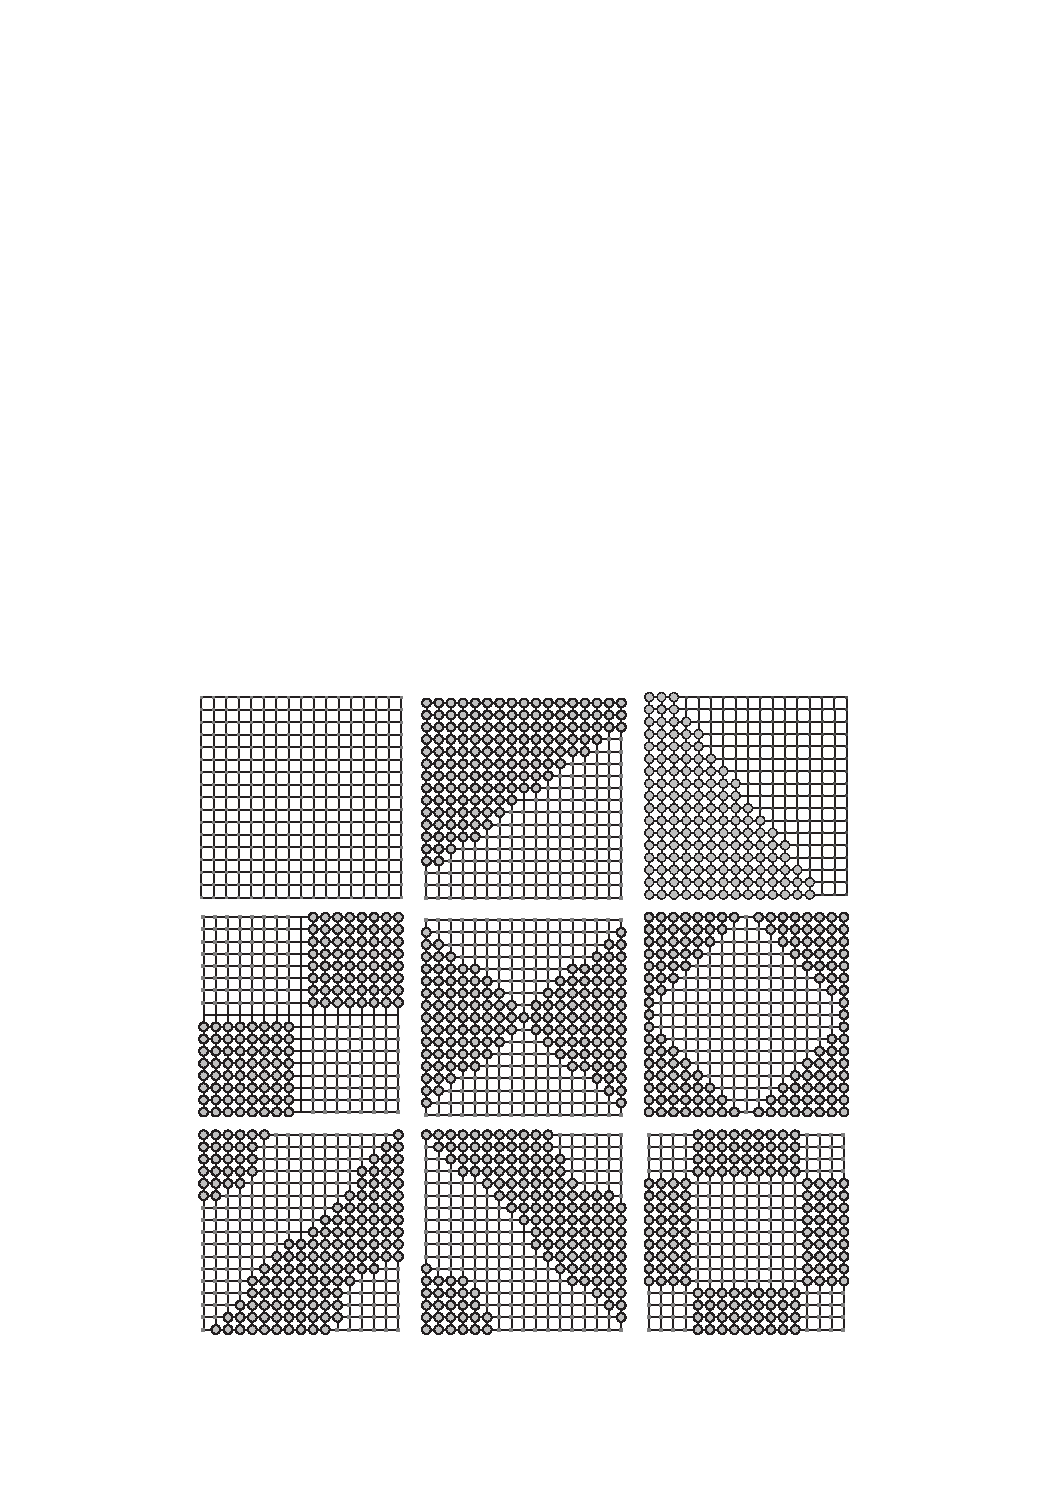
\includegraphics[width=0.70\textwidth]{Pozrikidis14_2-2-1}
  \caption{\label{fig:Pozrikidis14_2-2-1}
A $[17\times17]$ rectangular Helmholtz \refeq{Pozrikidis14(1.1.11H)}
network. Positive components of an eigenvector are marked as filled
circles, negative components are marked as dots, and zero components are
unmarked. The network shown consists of $N=17^2=289$ nodes connected by
$L=544$ links. The degree of the 4 corner nodes is 2, the 60 edge nodes
is 3, and 225 interior nodes is 4. Exact expressions for the eigenvalues
and eigenvectors of the Laplacian of the square network are discussed in
Pozrikidis Chapter 3. The first nine eigenvalues corresponding to the
eigenvectors shown here are $\lambda_i=0$, 0.0341 (double), 0.0681,
0.1351 (double), 0.1691 (double), and 0.2701.
Pozrikidis\rf{Pozrikidis14} Fig~2.2.1.
  }
\end{figure}
%%%%%%%%%%%%%%%%%%%%%%%%%%%%%%%%%%%%%%%%%%%%

In
spectral partitioning (a weighed
sum of eigenvectors of the Laplacian matrix)
%relies on the zero-mean property expressed by ,
roughly an equal number of eigenvector components with positive
and negative sign appear.
Eigenvector corresponding to the zero eigenvalue of the Laplacian matrix
is uniform over the nodes of a network; the eigenvector corresponding to
the zero eigenvalue is filled with ones. Orthogonality of the set of
eigenvectors requires that all other eigenvectors have mean zero, his
Eq.~(2.2.8). Higher eigenvectors partition the network into two or a
higher number of pieces (spectral partitioning). To partition a network,
we may group together nodes whose eigenvector components corresponding to
a specified eigenvalue have the same sign. The eigenvalue with the second
smallest magnitude, is chosen for division into two fragments, while
higher eigenvalues are chosen for division into a higher number of
fragments.

A network whose structure is isomorphic to that of a square lattice
consists of two intersecting one-dimensional arrays of links. A theorem
due to Fiedler\rf{Fiedler73,AndMor85} states that the eigenvectors of the
Laplacian matrix for certain types of boundary conditions are tensor
products of those of the constituent one-dimensional graphs, and the
eigenvalues are the sums of the eigenvalues of the Laplacian of the
constituent one-dimensional graphs. This property reflects the
separability of the discrete Laplace operator in Cartesian coordinates.

We need to understand \catlatt\ eigenmodes. If $s<2$ lattice is a spring
mattress, with spring constant $2-s$, what are the normal modes of the
$s>2$ \catlatt?
In the above he discusses the Helmholtz, $s=2$ Laplacian eigenmodes
case \refeq{Pozrikidis14(1.1.11H)}.

\item[2020-01-21 Predrag]
Fruchart, Zhou and Vitelli\rf{FrZhVi20}
{\em Dualities and non-{Abelian} mechanics} seems interesting.
The abstract:
``
Dualities are mathematical mappings that reveal links between apparently
unrelated systems in virtually every branch of physics.
Systems mapped onto themselves by a duality transformation are called
self-dual and exhibit remarkable properties, as exemplified by the scale
invariance of an Ising magnet at the critical point. Here we show how
dualities can enhance the symmetries of a dynamical matrix (or
Hamiltonian), enabling the design of metamaterials with emergent
properties that escape a standard group theory analysis. As an
illustration, we consider twisted kagome lattices,
reconfigurable mechanical structures that change shape by means of a
collapse mechanism. We observe that pairs of distinct configurations
along the mechanism exhibit the same vibrational spectrum and related
elastic moduli. We show that these puzzling properties arise from a
duality between pairs of configurations on either side of a mechanical
critical point. The critical point corresponds to a self-dual structure
with isotropic elasticity even in the absence of spatial symmetries and a
twofold-degenerate spectrum over the entire Brillouin zone. The spectral
degeneracy originates from a version of Kramers' theorem in which
fermionic time-reversal invariance is replaced by a hidden symmetry
emerging at the self-dual point. The normal modes of the self-dual
systems exhibit non-Abelian geometric phases that affect the
semiclassical propagation of wavepackets, leading to non-commuting
mechanical responses.
''

Mechanical structures are described at the linear level by normal modes
of vibration and their oscillation frequencies. Both are determined by
the dynamical matrix $\hat{D}$, which summarizes the Newton equations of motion
in the harmonic approximation [...] our analysis also applies
when $\hat{D}$ is replaced by other linear operators, such as the Maxwell
operator of a photonic crystal[ref28], the mean-field Hamiltonian of a quantum
system (in which case the eigenvalues are energies) or the dynamical
matrix of an electrical circuit\rf{NOSSS15,AlGlJi15,LIBBBMKT18}.

A \emph{symmetry} is a transformation that maps a system onto itself.
A \emph{duality} relates distinct models or structures.
In self-dual systems, the distinction between dualities and symmetries is
blurred: additional symmetries can emerge at a self-dual point even if
the spatial symmetries are unchanged.
Such dualities can be harnessed to engineer material properties from wave
propagation to static responses that are not predicted by a standard
symmetry analysis based on space groups.
    \index{symmetry}\index{duality}



This one as well:
Souslov and Vitelli\rf{SouVit19} {\em Geometry for mechanics}:
``
The mechanics of many materials can be modelled by a network of balls
connected by springs. A bottom-up approach based on differential geometry
now captures changes in mechanics upon network growth or merger, going
beyond the linear deformation regime.
''

\item[2021-01-09 Predrag]
Fruchart, Zhou and Vitelli\rf{FrZhVi20} cite

Ningyuan \etal\rf{NOSSS15}
{\em Time- and site-resolved dynamics in a topological circuit}:
I think we can ignore this paper. Though supplemental material explains:
(1) The Harper-Hofstadter model, and its extension to spinful systems.
(2) Photonic lattices, in both massive and massless limits.
(3) Adding topology to photonic lattice models.
(4) Mathematical tools for the calculation of band-structure,
corresponding band Chern numbers, and two-point response of photonic
lattice models.
(5) Mathematical tools for calculating band- and edge- structure of
finite strips.

Albert, Glazman and Jiang\rf{AlGlJi15}
{\em Topological properties of linear circuit lattices}
have a 3-site lattice example, where the Lagrangian contribution of the
link between neighboring sites is built from
a (kinetic) capacitive part with what we call {\jacobianOrb} \jMorb,
and a (potential)
inductive part with what we call shift matrix $\shift$.

\item[2021-01-09 Predrag]
Fruchart, Zhou and Vitelli\rf{FrZhVi20} cite
Lee \etal\rf{LIBBBMKT18} {\em Topolectrical circuits}.
The normal mode frequency matrix of our circuit is unitarily equivalent
to the hopping matrix of a quantum spin Hall insulator.

Circuits consisting of resistor, inductor and capacitor (RLC) components
are governed by its circuit Laplacian, which is analogous to the
Hamiltonian describing the energetics of a physical system. Here we show
that topological insulating and semimetallic states can be realized in a
periodic RLC circuit.

Any electrical circuit network can be represented by a graph whose nodes
and edges correspond to the circuit junctions and connecting
wires/elements. The circuit behavior is fundamentally described by
Kirchhoff's law. As an initial step towards identifying circuits with
tight-binding lattice models, they rewrite Kirchhoff's law in a matrix
form, and consider circuits made up of periodic sublattices, with
periodic boundary conditions (i.e. without grounded terminations).

What we call {\jacobianOrb} \jMorb\ they call `the grounded Laplacian'
$\jMorb$.

The regularized inverse of $\jMorb$ known as the circuit Green's function
(regularization in this context means that 0 modes are omitted).
The Laplacian is defined in terms of the conductances by $L=D-C$,
where $C$ is the (adjacency) matrix of conductances and
$D$ lists the total conductances out of each node.
They call the set of eigenvalues the bandstructure of the circuit, and
also refer to the nodes as sites.

RLC circuits obey a linear 2nd order ordinary differential equation
(ODE), just like a mechanical system with springs, dampers and masses.






\end{description}

\renewcommand\speriod[1]{{\ensuremath{L_{#1}}}}  %continuous spatial period
\renewcommand\period[1]{{\ensuremath{T_{#1}}}}  %continuous time period
